% Created 2018-03-10 sob 00:49
% Intended LaTeX compiler: pdflatex
\documentclass[11pt]{article}
\usepackage[utf8]{inputenc}
\usepackage[T1]{fontenc}
\usepackage{graphicx}
\usepackage{grffile}
\usepackage{longtable}
\usepackage{wrapfig}
\usepackage{rotating}
\usepackage[normalem]{ulem}
\usepackage{amsmath}
\usepackage{textcomp}
\usepackage{amssymb}
\usepackage{capt-of}
\usepackage{hyperref}
\usepackage[, slovene]{babel}
\usepackage[a4paper, left=2.5cm, right=2.5cm, top=2.5cm, bottom=2.5cm]{geometry}
\setlength{\parindent}{0cm}
\author{Gregor Nemec}
\date{07.03.2018}
\title{Prometna signalizacija}
\hypersetup{
 pdfauthor={Gregor Nemec},
 pdftitle={Prometna signalizacija},
 pdfkeywords={},
 pdfsubject={},
 pdfcreator={Emacs 25.3.1 (Org mode 9.1.7)}, 
 pdflang={Slovene}}
\begin{document}

\maketitle

\section{Naloga}
\label{sec:orgb55e861}
S signalizacijo v prometu se srečujemo vsak dan. Naš končni cilj je prehod za
pešce za slepe in slabovidne.

\section{Sestavine}
\label{sec:org96f8664}
Pri projektu bomo potrebovali:
\begin{itemize}
\item 1x prototipna plošča,
\item 1x razširitev in podaljševalni kabel GPIO pinov,
\item 5x LED dioda (2x rdeča, 2x zelena, 1x rdeča),
\item 5x \(220 \Ohm\) upornik,
\item 1x piskač (buzzer)
\item 1x gumb,
\item več veznih žičk različnih barv.
\end{itemize}

\section{Vezje}
\label{sec:org55ca055}
Na spodnji sliki je končna slika ciljnega vezja signalizacije. 

\begin{figure}[htbp]
\centering
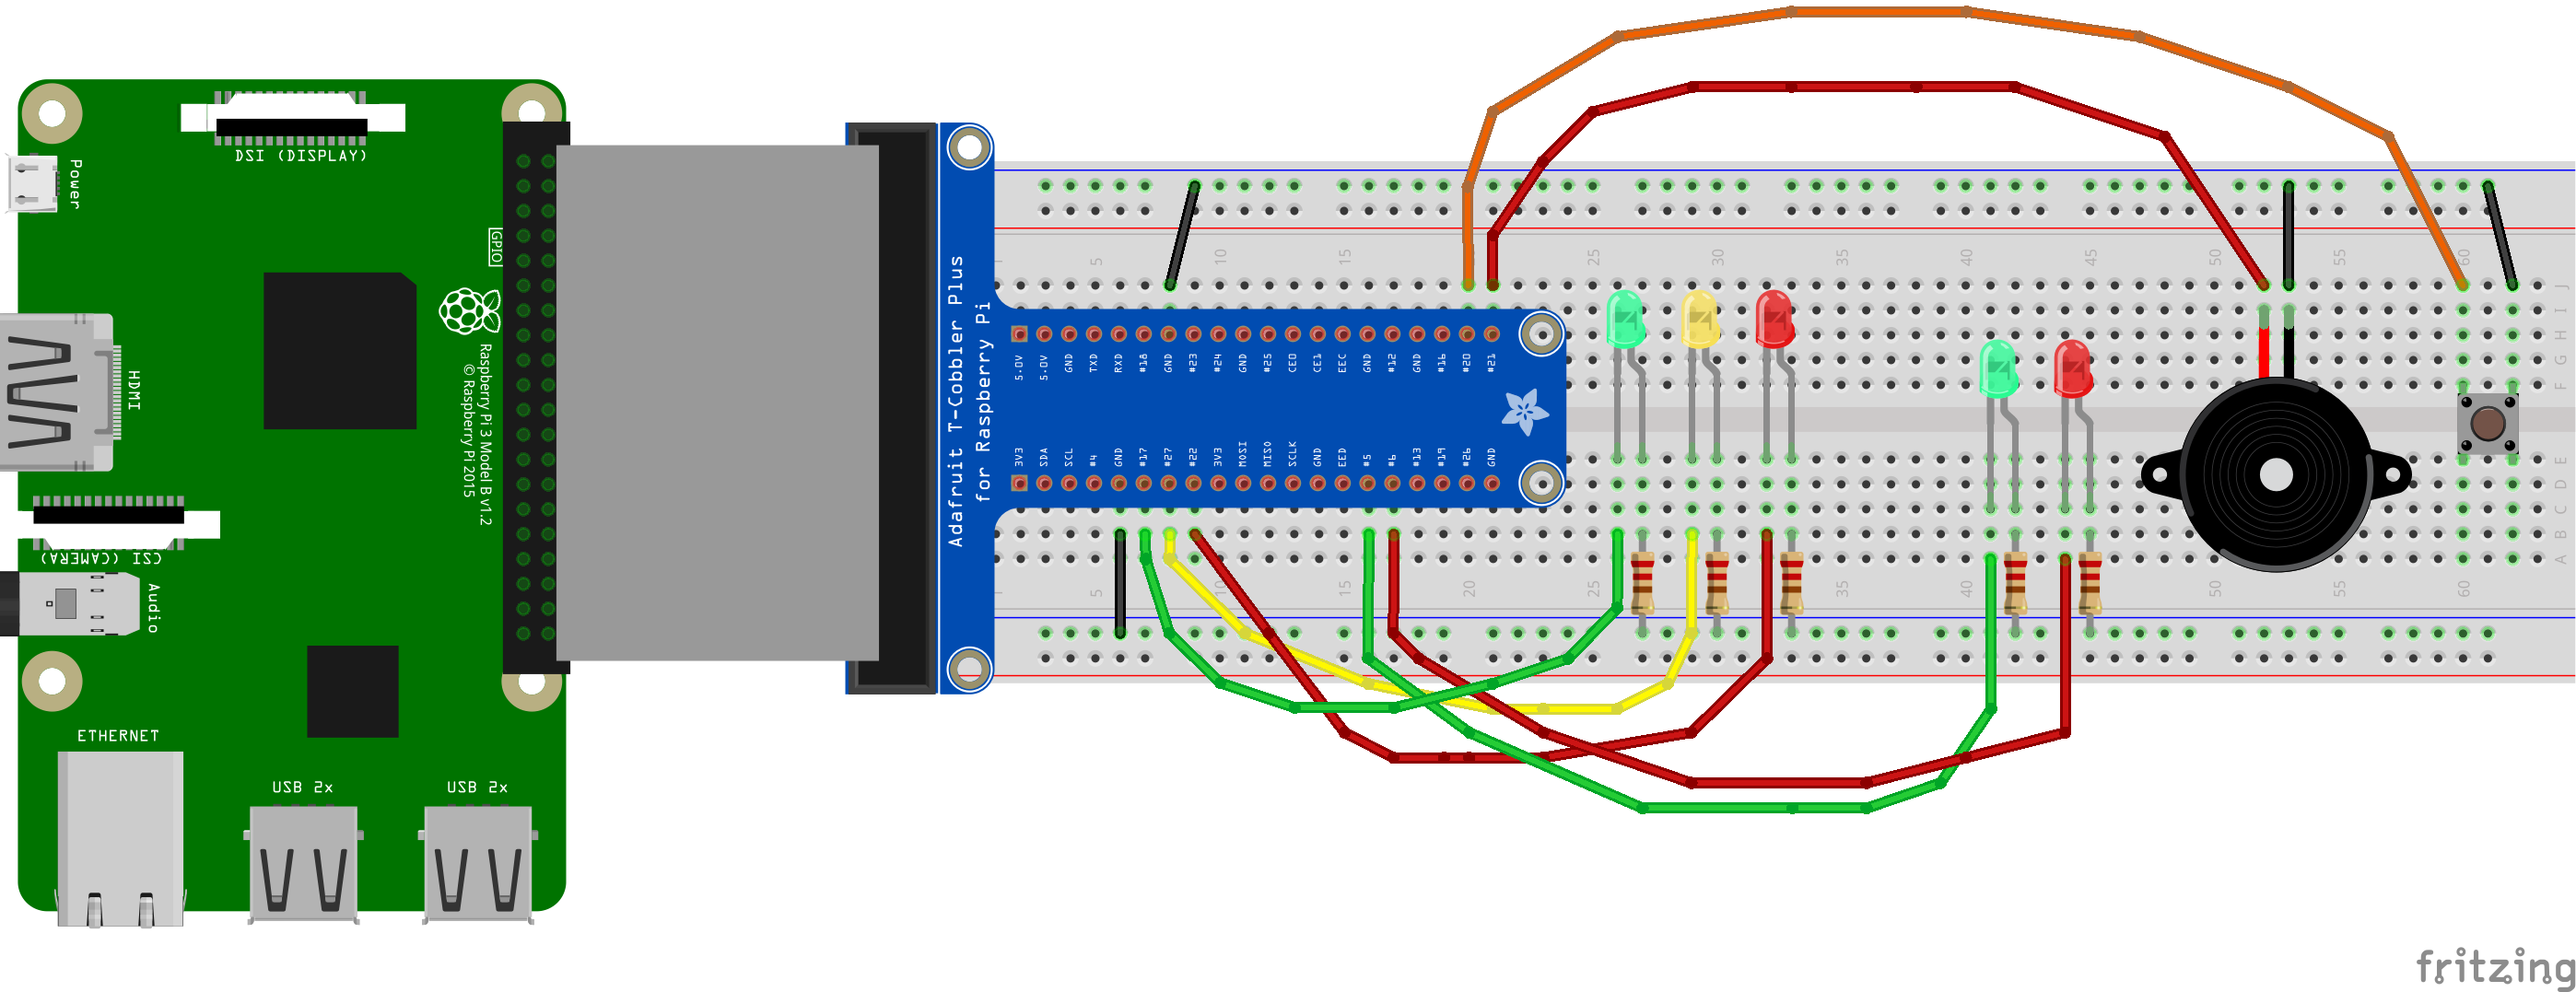
\includegraphics[width=.9\linewidth]{breadboard/REB_RES_3LEDsem_2LED_sem_BT_BUZ_bb.png}
\caption{\label{fig:orgb45d077}
Končna slika vezja z vsemi elementi}
\end{figure}

\section{Koraki izdelave}
\label{sec:orgcaf9849}

\subsection{Priklop Raspbery-Pi}
\label{sec:orge86a000}

\subsection{Spoznavanje Pixle in IDLE}
\label{sec:org789a045}
V tem delu bomo spoznali uporabniški vmesnik \textbf{PIXLE} in urejevalnik besedil
za programiranje \textbf{Thonny}.

\subsection{Spoznavanje elektrotehničnih elementov}
\label{sec:org7030264}

\subsubsection{Prototipna ploščica}
\label{sec:orgf177563}

\subsubsection{Upornik}
\label{sec:org678c60f}

\subsubsection{LED dioda}
\label{sec:org71f6d16}

\subsubsection{Stikalo}
\label{sec:org14439ec}

\subsubsection{Piskač}
\label{sec:org5efb436}


\subsection{GPIO}
\label{sec:orgea43536}

\subsection{Priklop razširitvenega priklopa na prototipno ploščico in R-Piska}
\label{sec:orgd6ffdc7}
Pred sabo imaš prototipno ploščico in na njo vključen razširitveni priklop.
Ta nam omogoča samo podaljšek, tako do posameznih pinov GPIO pridemo
neposredno na prototipni ploščici, kar nam omogoča nekoliko lažje delo.

\subsection{Utripajoča led (1x)}
\label{sec:org974b864}
Pri tej nalogi bomo spoznali kako priklopimo eno LED diodo v vezje in jo
krmilimo tako, da bo ta utripala. 
\subsubsection{Vezava LED}
\label{sec:orgb6fdc8c}
\begin{figure}[htbp]
\centering
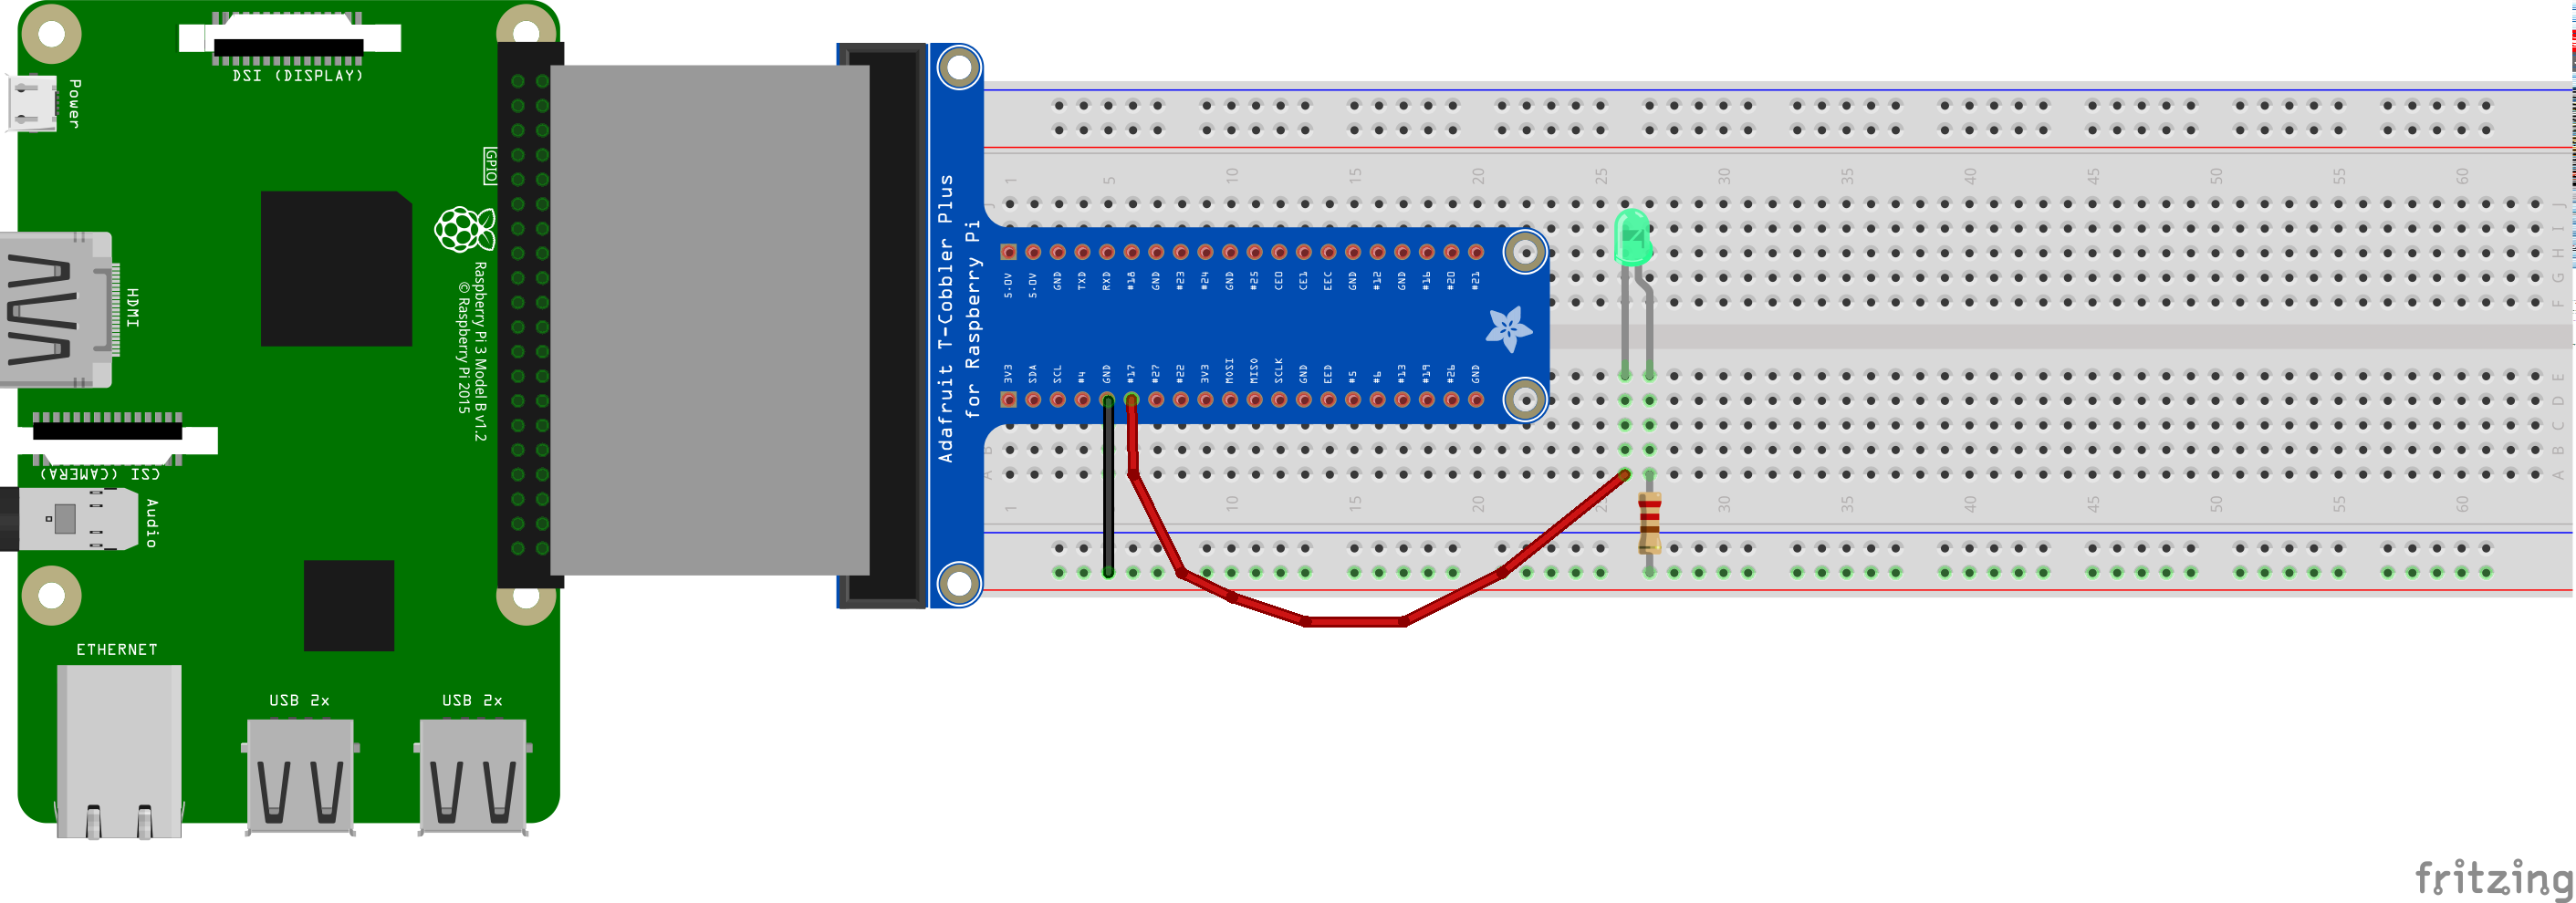
\includegraphics[width=.9\linewidth]{breadboard/REB_1LED.png}
\caption{\label{fig:orgbb0710a}
Vezje z eno LED diodo.}
\end{figure}

\subsubsection{Programska koda}
\label{sec:org6667134}
Za delovanje programa bomo potrebovali dve zunanjivi knjižnici \textbf{gpiozero} in
\textbf{time}. \textbf{gpiozreo} bo poskrbela da bomo lahko prižigali in ugašali lučke.
Knjižnica \textbf{time} bo poskrbela za pavze. V programu za urejanje programske
kode odpri datoteko semafor\(_{\text{pesci}}\)\(_{\text{zacetek.py}}\). V \textbf{Thonny} odprite spodnjo
datoteko.

\textbf{DATOTEKA}: \texttt{code/01\_led.py}

\begin{verbatim}
import gpiozero
import time

#inicializacija LED diode 
led = gpiozero.LED(27) #GPIO povemo, da imamo LED priklopljeno na pinu 27.

while True:            #Zanka, ki se neskončno ponavlja.
    led.on()           #Z ukazom on() prižgemo LED.
    print("LED on")    #Izpis v ukazno vrstico ali lupino.
    time.sleep(1)      #Zaspi za čas v sekundah.
    led.off()          #Z ukazom off() ugasnemo LED.
    print("LED off")
    time.sleep(1)
\end{verbatim}

\subsubsection{Vaja}
\label{sec:org0a7136d}
Program spremeni tako, da bodo lučke utripale počasneje ali hitreje. 

\subsection{Semafor za pešce (2x LED vzporedno)}
\label{sec:org4e06ec3}
Sestavimo vezje rdeče in zelene barve ter jih programirajmo tako, da bodo
simulirale prehod za pešce. 
\subsubsection{Vezje}
\label{sec:orge07d7f8}

\begin{figure}[htbp]
\centering
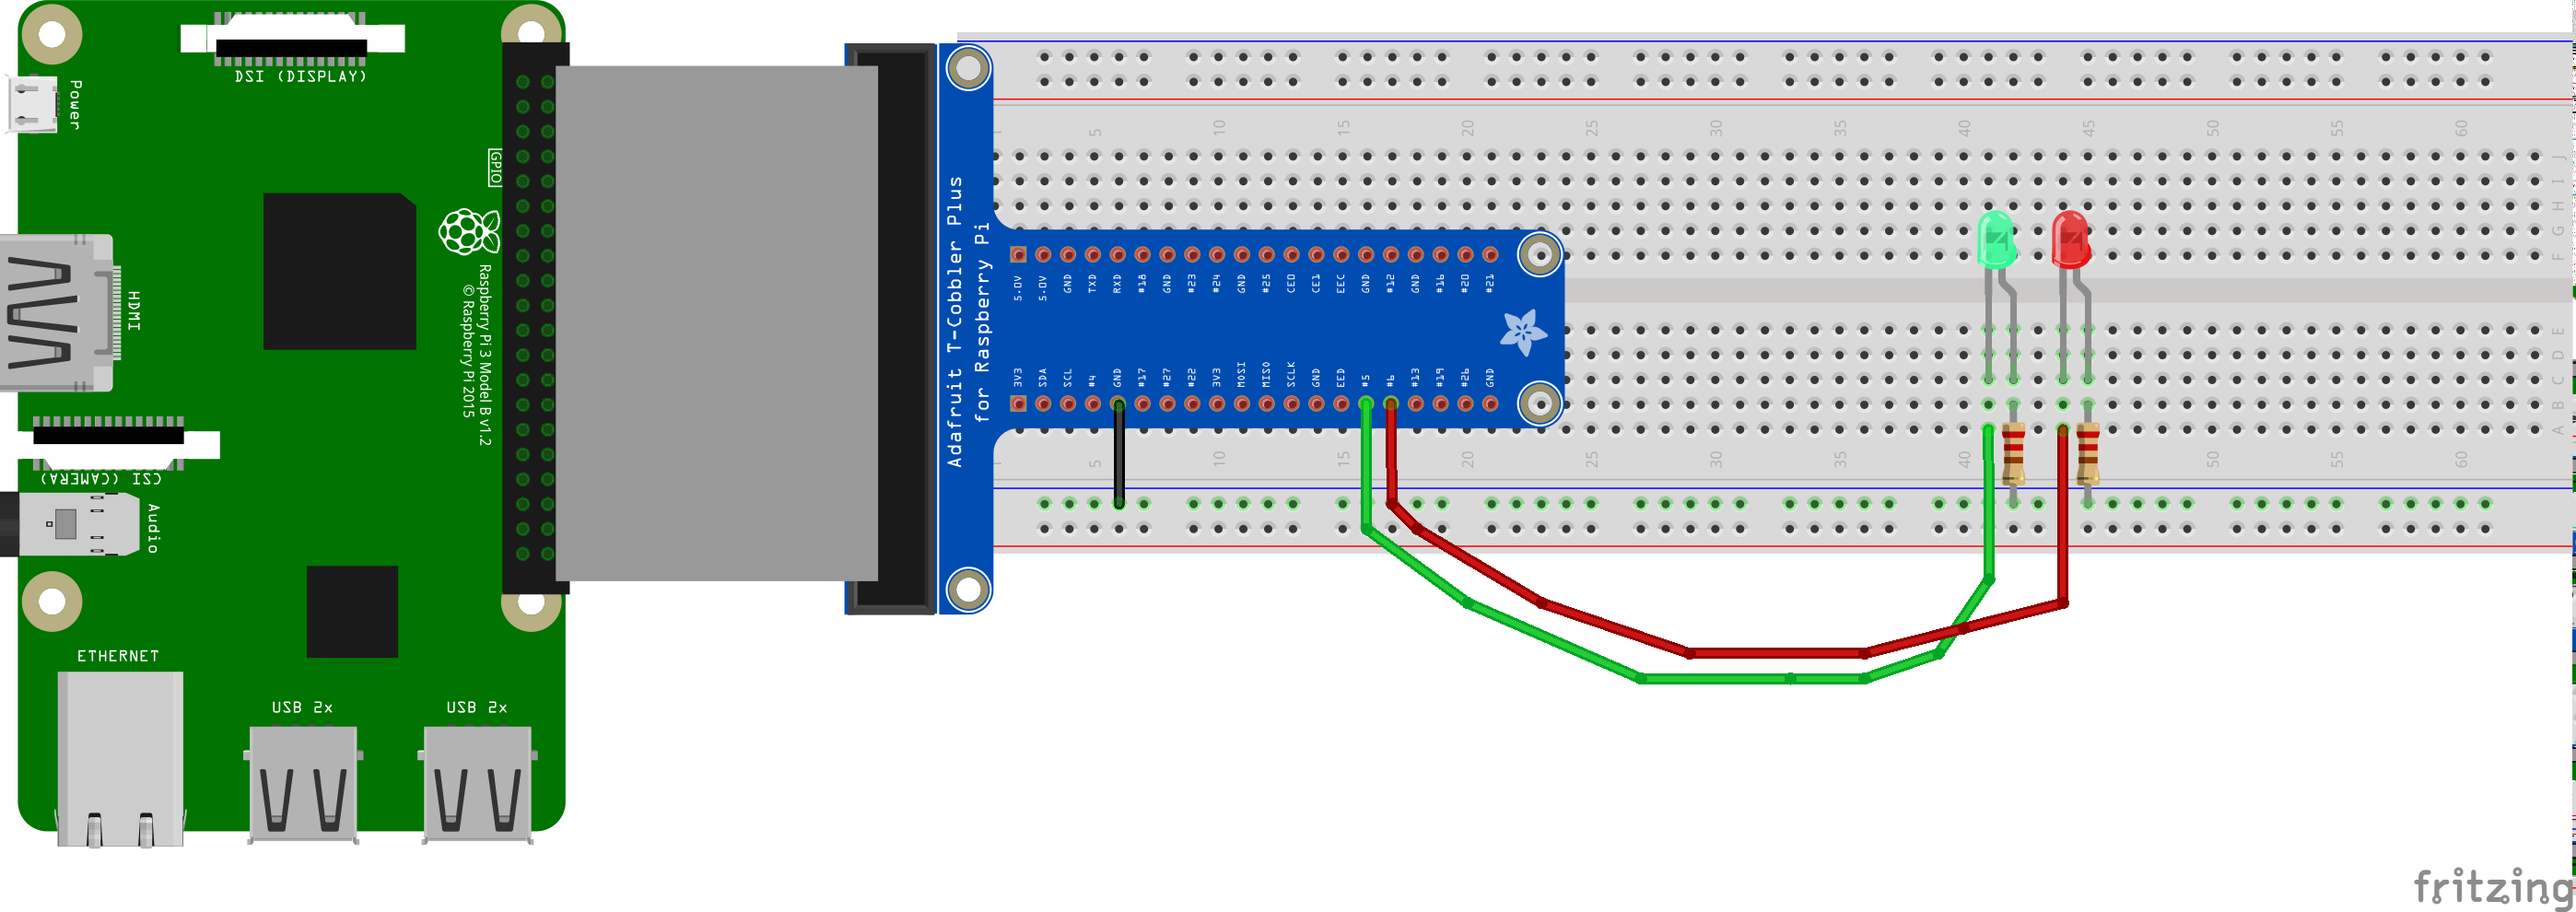
\includegraphics[width=.9\linewidth]{breadboard/REB_2LED_sem.png}
\caption{\label{fig:org878b012}
Vezava 2x LED za semafor za peščce}
\end{figure}

\subsubsection{Programska koda}
\label{sec:org7d24e99}
Program od prej spremeni na naslednji način. 
\begin{enumerate}
\item Naredi inicializacijo dveh spremenljivka za dve LED diodi, eno za zeleno
in drugo za rdečo.
\item V \texttt{while True:} zanko zapiši delovanje semaforja v naslednjih korakih: 
rdeča prižgana
zelena ugasnjena
počakaj 3 s

rdeča ugasnjena
zelena prižgana
počakaj 1 s
\end{enumerate}

\textbf{DATOTEKA}: \texttt{code/02\_semafor\_pesci.py}

\begin{verbatim}
#inicializacija semafor pešci
p_zelena = gpiozero.LED(5)
p_rdeca = gpiozero.LED(6)

while True:
    p_rdeca.on()
    p_zelena.off()
    time.sleep(3)

    p_rdeca.off()
    p_zelena.on()
    time.sleep(1)
\end{verbatim}

\subsection{Semafor za avtomobile (3x led zaporedno)}
\label{sec:org20b915a}
K obstoječemu vezju dodamo vezje semaforja za avtomobile.

\subsubsection{Vezje}
\label{sec:org53952da}
\begin{figure}[htbp]
\centering
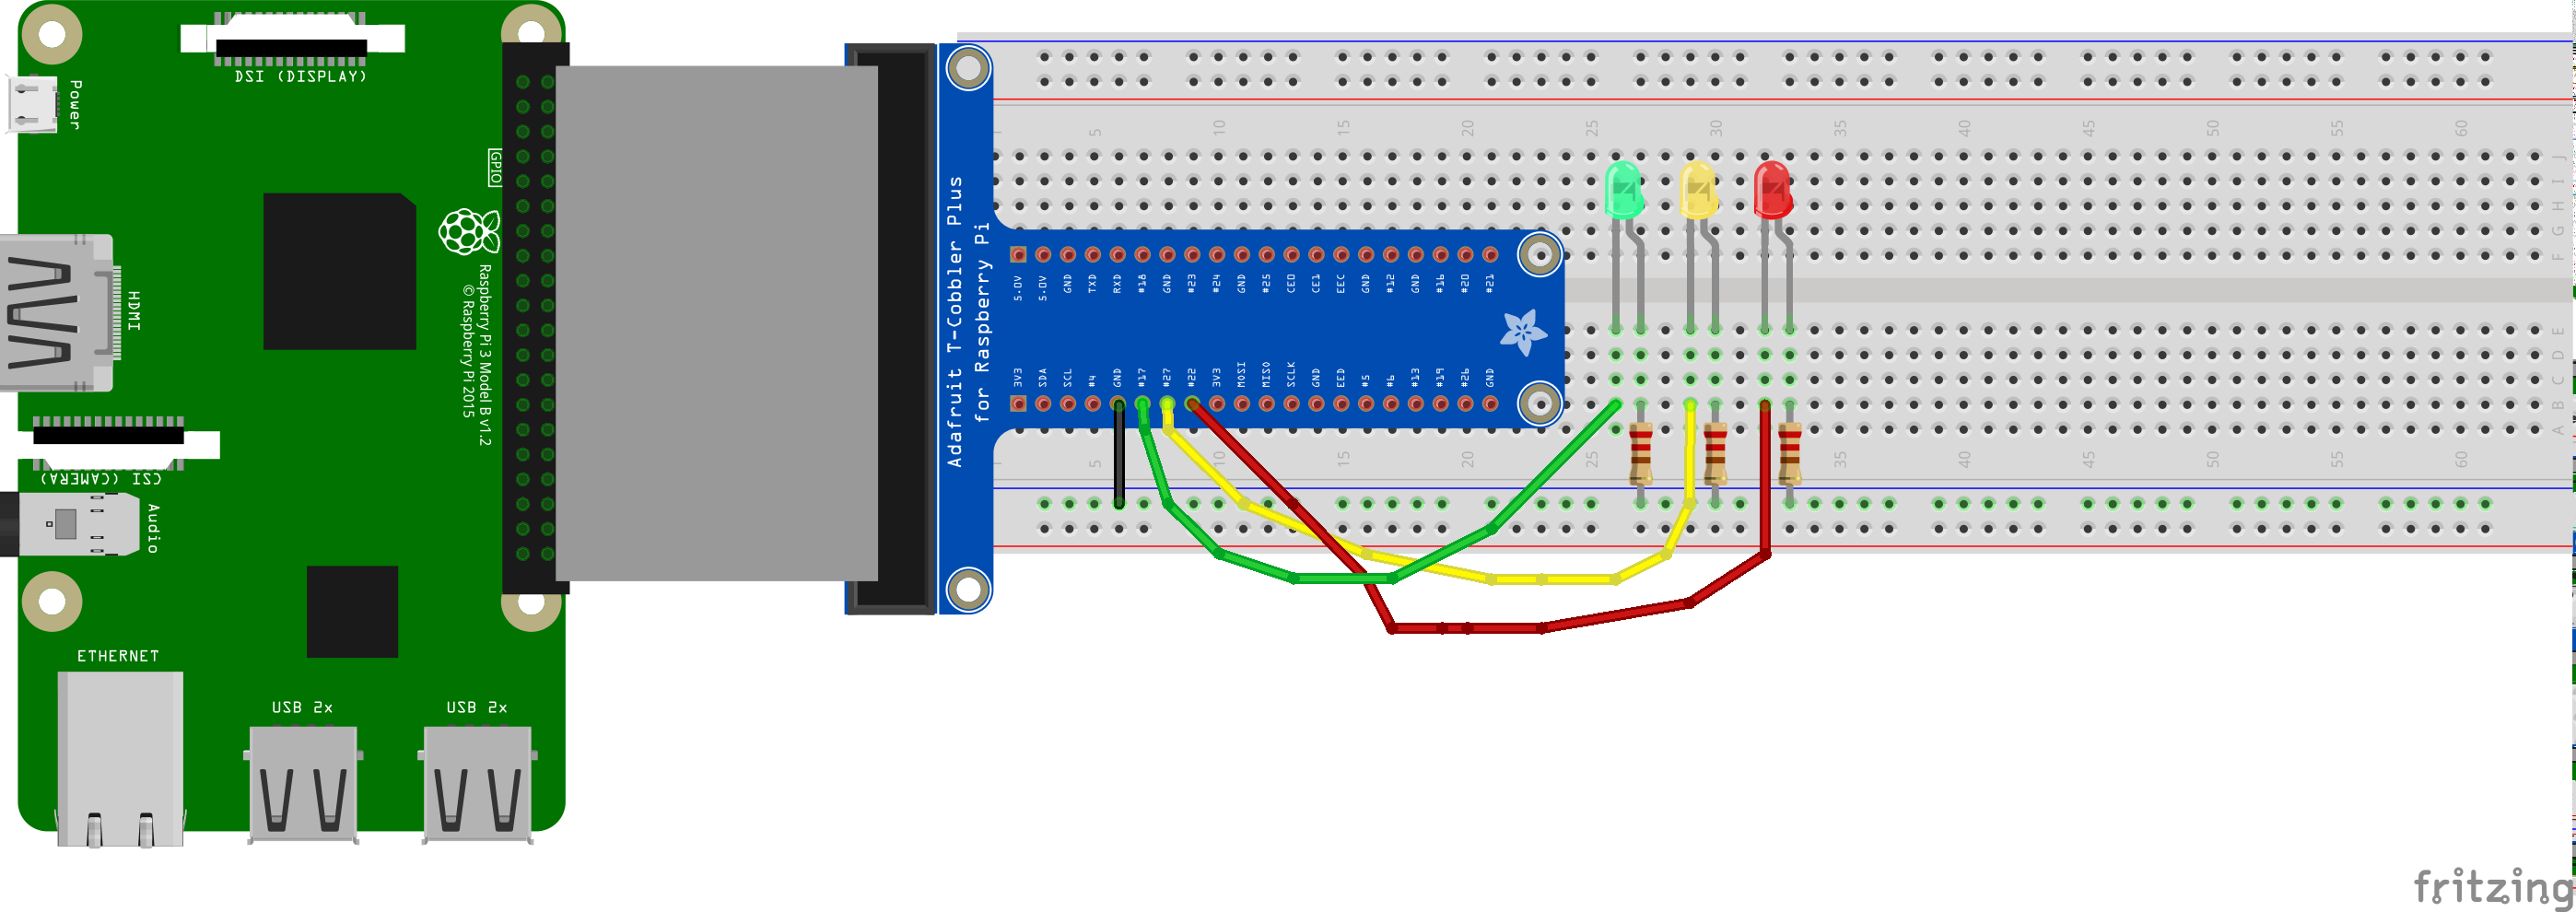
\includegraphics[width=.9\linewidth]{breadboard/REB_3LED_sem.png}
\caption{\label{fig:org7fd27d4}
Vezava 2x LED za semafor za peščce}
\end{figure}

\subsubsection{Programska koda}
\label{sec:org6c447a1}
\begin{verbatim}
import gpiozero
import time

#SEMAFOR AVTOMOBILI
#Inicializacija
a_zelena = gpiozero.LED(17)
a_oranzna = gpiozero.LED(27)
a_rdeca = gpiozero.LED(22)

while True:
    a_rdeca.on()
    a_oranzna.off()
    a_zelena.off()
    time.sleep(3)

    a_oranzna.on()
    time.sleep(1)

    a_rdeca.off()
    a_oranzna.off()
    a_zelena.on()
    time.sleep(3)

    a_oranzna.on()
    a_zelena.off()
    time.sleep(1)
\end{verbatim}

\subsection{Priklop stikala in priklop piskača}
\label{sec:org20ddcdd}
V tem delu bomo priklopili gumb in z njim krmilili vklop semaforja za pešce.

\subsubsection{Vezava}
\label{sec:org8c90177}
Piskača priklopimo posebej na povezave \textbf{GPIO21}, gumb na povezavo \textbf{GPIO22}
in ozemljitev \textbf{GND}. 

Glej končno sliko.

\subsubsection{Programska koda}
\label{sec:org69120d0}
\begin{verbatim}
#Inicializacija piskača
zvok = gpiozero.Buzzer(20)
#Inicializacija gumba
gumb.Button(21)

#Uporaba zanka in pogojnega stavka za preveranje stanja tipke.
while True:
    if gumb.is_pressed:    #Z pogojnim stavkom preverjamo če je gumb pritisnjen. 
        zvok.on()          #vklop zvoka
        time.sleep(0.5)
    else:
        zvok.off()         #Izklop zvoka
        time.sleep(0.5)
\end{verbatim}

\subsection{Končni projekt}
\label{sec:org42f7cc0}
Sedaj imamo priklopljene vse elemente. Napisati moramo samo še program, ki 
bo poganjal simulacijo semaforja. 

\subsubsection{Programska koda}
\label{sec:org5b9a69a}


\subsubsection{Vezje}
\label{sec:orgb9d6900}
\begin{figure}[htbp]
\centering
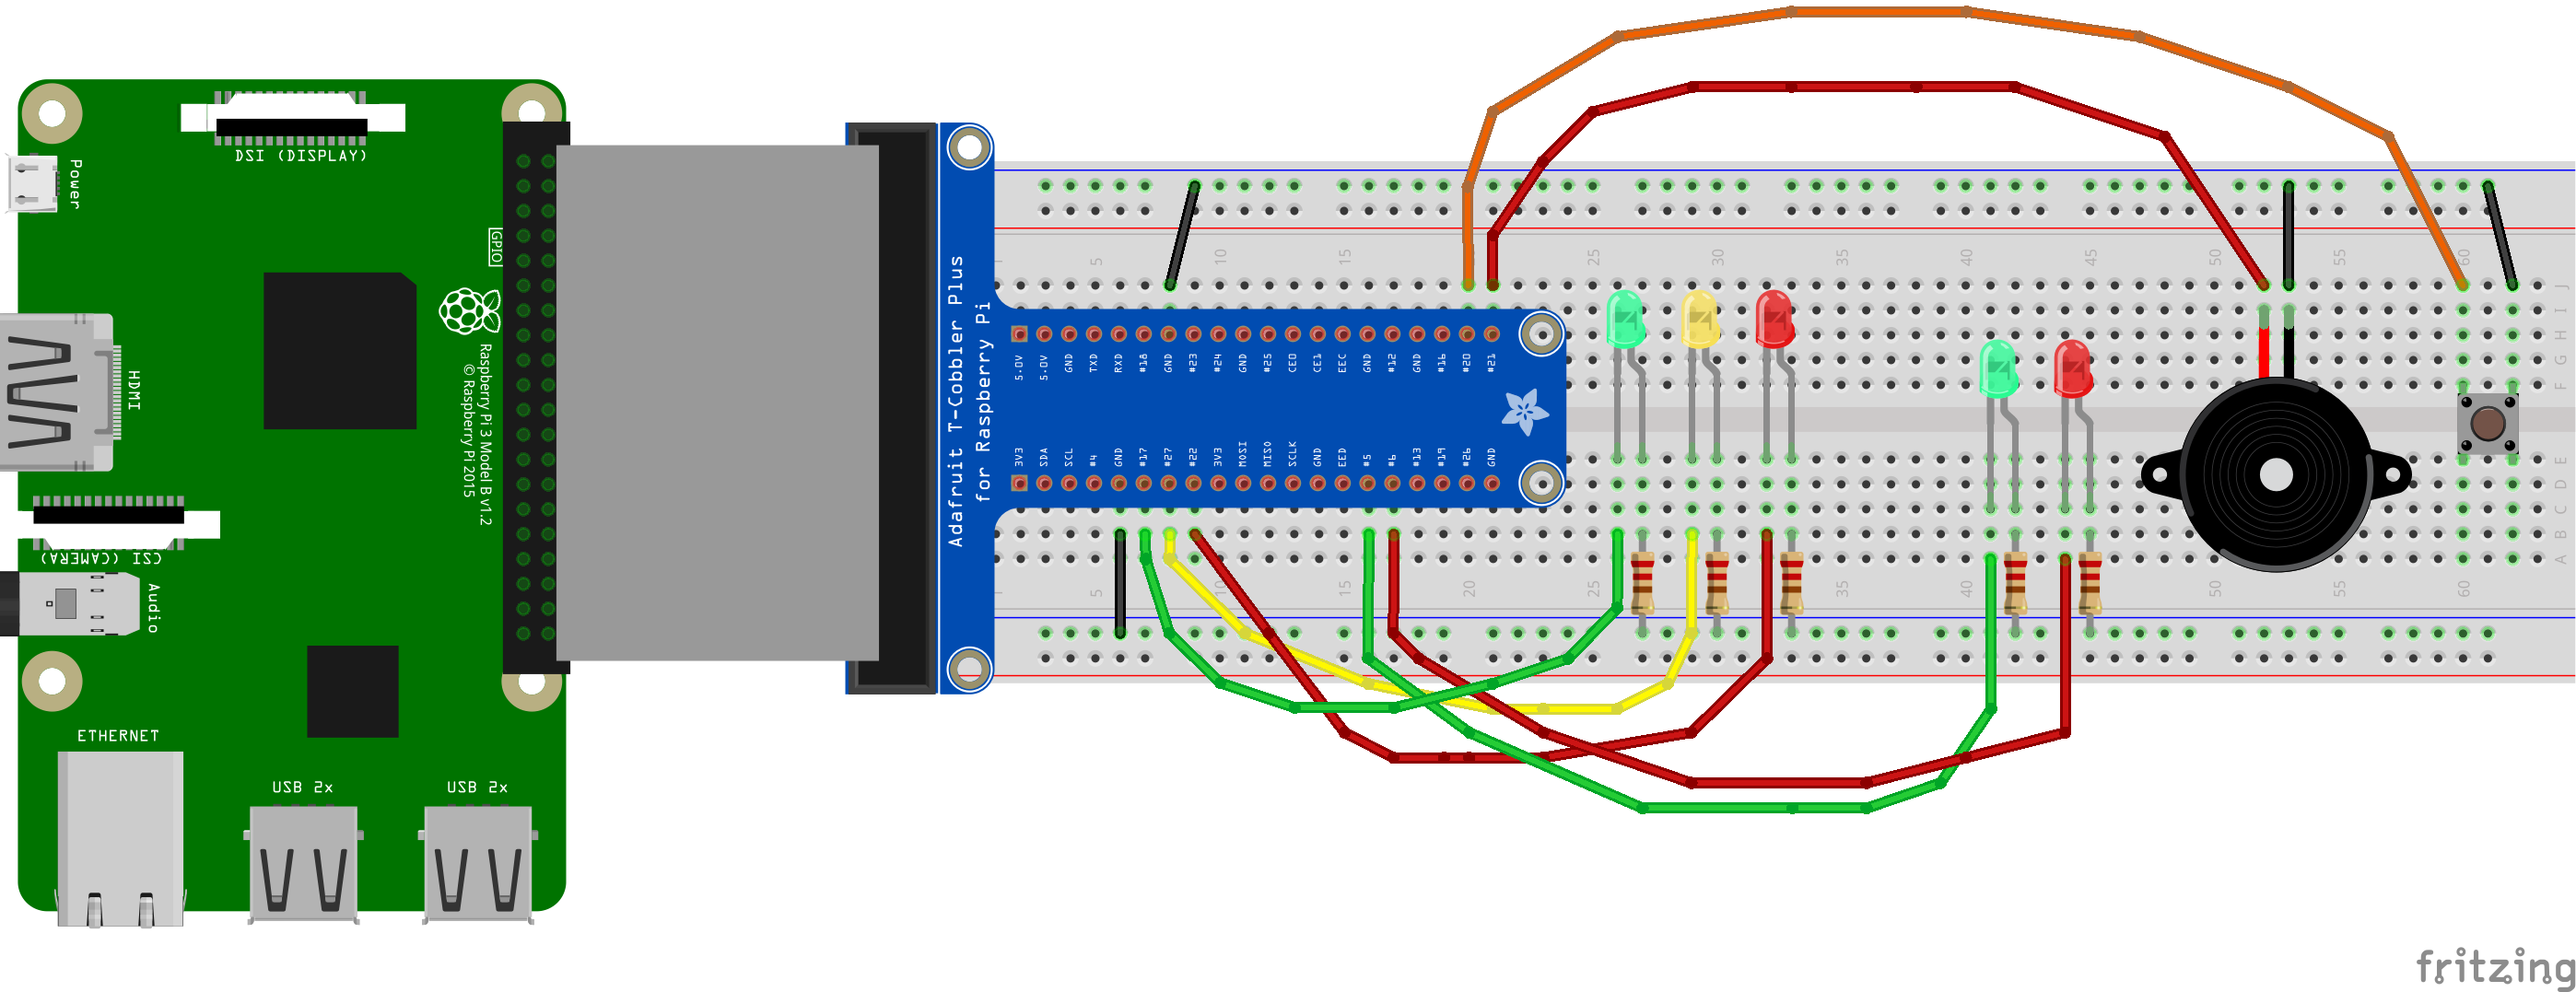
\includegraphics[width=.9\linewidth]{breadboard/REB_RES_3LEDsem_2LED_sem_BT_BUZ_bb.png}
\caption{\label{fig:orgaddee64}
Končna vezava vseh elementov.}
\end{figure}

\subsubsection{Programska koda}
\label{sec:orga6a5831}
\begin{verbatim}
#!/usr/bin/env python
# -*- coding: utf-8 -*-

import gpiozero
import time

#SEMAFOR AVTOMOBILI
#Inicializacija semafor avtomobili
a_zelena = gpiozero.LED(17)
a_oranzna = gpiozero.LED(27)
a_rdeca = gpiozero.LED(22)

#inicializacija semafor pešci
p_zelena = gpiozero.LED(5)
p_rdeca = gpiozero.LED(6)

#Inicializacija piskača
zvok = gpiozero.Buzzer(20)
#Inicializacija gumba
gumb = gpiozero.Button(21)

def prehod():
    time.sleep(2)
    #oranzna za avtomobile
    a_zelena.off()
    a_oranzna.on()
    time.sleep(1)
    #rdeca za avtomobile
    a_oranzna.off()
    a_rdeca.on()
    time.sleep(1)
    #zelena za pesce
    p_rdeca.off()
    p_zelena.on()
    zvok.on()
    time.sleep(2)
    #rdeca za pesce
    zvok.off()
    p_zelena.off()
    time.sleep(0.5)
    p_rdeca.on()
    a_oranzna.on()
    a_rdeca.off()
    time.sleep(1)
    a_zelena.on()
    a_oranzna.off()

a_rdeca.off()
a_oranzna.off()
a_zelena.on()

p_rdeca.on()
p_zelena.off()

while True:
     if gumb.is_pressed:
         print("Pritisnil!")
         prehod()

\end{verbatim}

\section{Viri in Literatura}
\label{sec:orgbb2c851}
\begin{enumerate}
\item Gregor Anželj, \textbf{Prometna signalizacija}, 
\url{https://anzeljg.github.io/rpi/rpi/3201/index.html}
\end{enumerate}
\end{document}
